% Biography section
\newcommand{\biospace}{\vspace{-2em}}
\biospace
\begin{IEEEbiography}[{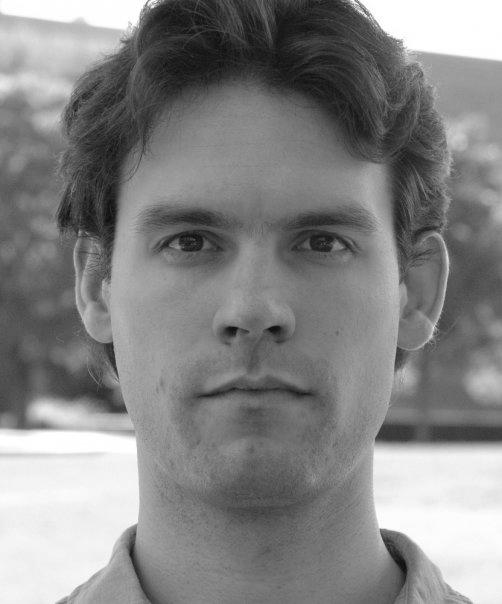
\includegraphics[width=1in,height=1.25in,clip,keepaspectratio]{bios/drew}}]{Andrew Wagner}
received his Bachelor's degree in General Engineering in 2003,
and his Master's degree in Electrical Engineering in 2006, from the University
of Illinois at Urbana-Champaign, where he is currently a Ph.D.
candidate in Electrical \& Computer Engineering.
His research interests include robotics, computer vision, and optimal control.
His recent work focuses on parallel algorithms for sparsity
based face recognition.\end{IEEEbiography}

\biospace
\begin{IEEEbiography}[{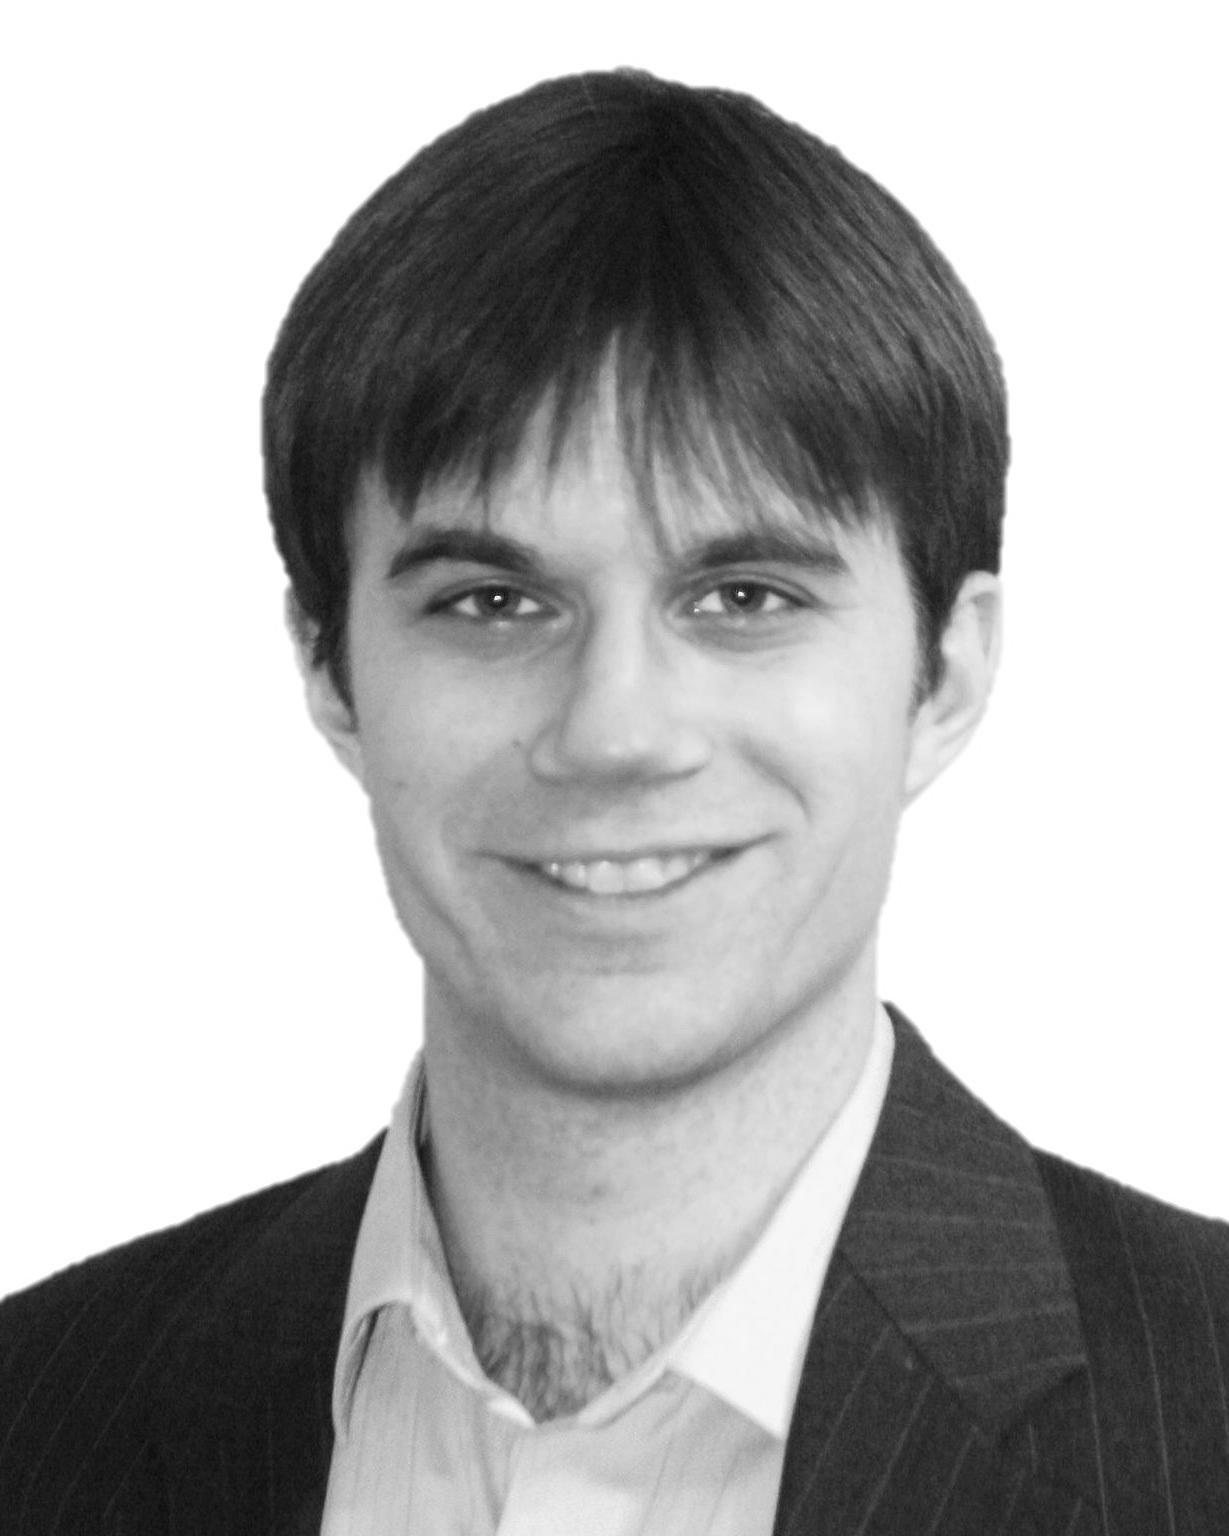
\includegraphics[width=1in,height=1.25in,clip,keepaspectratio]{bios/john}}]{John
Wright} received his PhD in Electrical Engineering from the
University of Illinois at Urbana-Champaign in October 2009. He is currently a
researcher in the Visual Computing group at Microsoft Research Asia.  His
research focuses on developing provably correct and efficient tools for
recovering low-dimensional structure in corrupted high-dimensional datasets.
His work has received a number of awards, including the 2009 Lemelson-Illinois
Prize for Innovation, the 2009 UIUC Martin Award for Excellence in Graduate
Research, a 2008-2010 Microsoft Research Fellowship, a Carver fellowship, and a
UIUC Bronze Tablet award.  \end{IEEEbiography}

\biospace
\begin{IEEEbiography}[{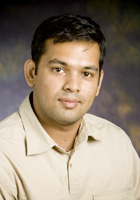
\includegraphics[width=1in,height=1.25in,clip,keepaspectratio]{bios/arvind}}]{Arvind Ganesh}
received his Bachelor's and Master's degrees, both in Electrical
Engineering, from the Indian Institute of Technology, Madras, India in 2006. He
is currently a PhD candidate in the Electrical \& Computer Engineering
Department at the University of Illinois, Urbana-Champaign. His research
interests include compressed sensing, computer vision, and machine learning.
His recent work focuses on low-rank matrix recovery techniques for
batch image alignment and texture rectification.  \end{IEEEbiography}

\biospace
\begin{IEEEbiography}[{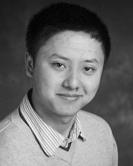
\includegraphics[width=1in,height=1.25in,clip,keepaspectratio]{bios/zihan}}]{Zihan Zhou}
Zihan Zhou received the bachelor's degree in automation from Tsinghua
University, China, in 2007. Since then, he has been with University of Illinois
at Urbana-Champaign, where he received the MS degree in electrical and computer
engineering and where he is now working toward the PhD degree. During the
summer of 2009, he was a research intern with Microsoft Research Asia, Beijing.
His research interests include computer vision, signal processing and machine
learning. He is a student member of the IEEE.
\end{IEEEbiography}

\biospace
\begin{IEEEbiography}[{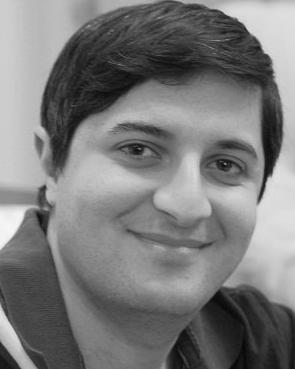
\includegraphics[width=1in,height=1.25in,clip,keepaspectratio]
{bios/hossein}}]{Hossein Mobahi} received his Bachelor's and Master's degrees
in Iran, both in Computer Engineering from Azad University (Tehran-South) in
2003  and University of Tehran in 2005 respectively. He is currently a PhD
candidate in the Computer Science Department at the University of Illinois,
Urbana-Champaign. His research interests include pattern classification,
clustering and optimization.  His recent research focuses on iterative
smoothing for image alignment.  \end{IEEEbiography}

\biospace
\begin{IEEEbiography}[{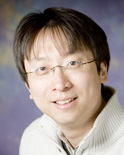
\includegraphics[width=1in,height=1.25in,clip,keepaspectratio]{bios/yi}}]{Yi
Ma} received two Bachelors degree in Automation and Applied Mathematics
from  Tsinghua University, Beijing, China, in 1995. He received an Master
degree in Electrical Engineering and Computer Sciences (EECS) in 1997, a second
Master degree in Mathematics in 2000, and the Ph.D. degree in EECS in 2000, all
from the University of California at Berkeley. He is currently an associate
professor (with tenure) at the Department of Electrical and Computer
Engineering, University of Illinois at Urbana-Champaign, and since January 2009
has also served as research manager for the Visual Computing Group at Microsoft
Research Asia, Beijing, China.  \end{IEEEbiography}
\vfill

% You can push biographies down or up by placing
% a \vfill before or after them. The appropriate
% use of \vfill depends on what kind of text is
% on the last page and whether or not the columns
% are being equalized.


% Can be used to pull up biographies so that the bottom of the last one
% is flush with the other column.
%\enlargethispage{-5in}
